\begin{figure}[h]
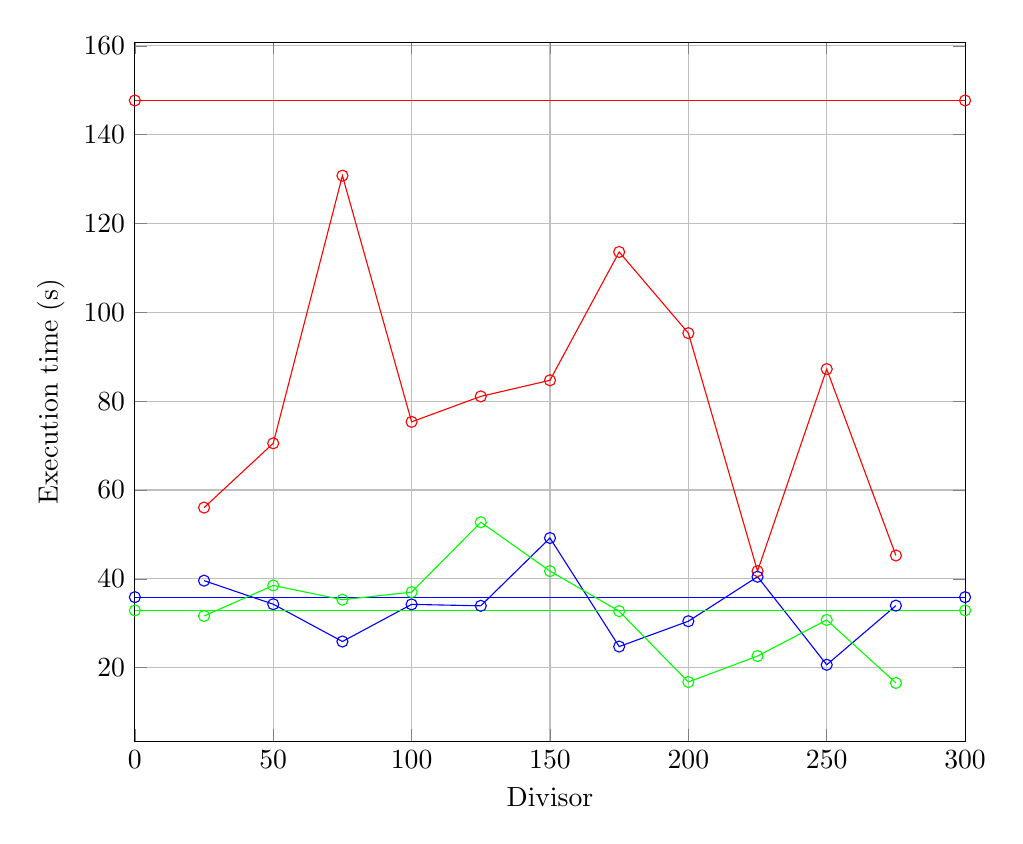
\begin{tikzpicture}
\begin{axis}[%
	grid=both,
	width=\textwidth,
	ylabel=Execution time (s),
	xlabel=Divisor,
	xmin=0,
	xmax=300,
	scatter/classes={%
    a={mark=o,draw=red}, 
    b={mark=o,draw=blue}, 
    c={mark=o,draw=green}}]
    
    
    %%% Instance 1
\addplot[scatter,color=red,
    scatter src=explicit symbolic]%
table[meta=label] {
x y label
0 147.68719898 a
300 147.68719898 a 
};
\addplot[scatter,color=red,%
    scatter src=explicit symbolic]%
table[meta=label] {
x y label
25 56.035697301 a
50 70.506202712 a
75 130.764253137 a
100 75.343499411 a
125 81.077518782 a
150 84.697921336 a
175 113.591657869 a
200 95.3119617 a
225 41.735343725 a
250 87.221499713 a
275 45.258815257 a
};
    %%% Instance 2
\addplot[scatter,color=blue,
    scatter src=explicit symbolic]%
table[meta=label] {
x y label
0 	35.87421779 b
300 	35.87421779 b 
}; 

\addplot[scatter,color=blue,%
    scatter src=explicit symbolic]%
table[meta=label] {
x y label
25 39.589334114 b
50 34.289058978 b
75 25.889187605 b
100 34.247770167 b
125 33.923824248 b
150 49.188483845 b
175 24.751333733 b
200 30.455340901 b
225 40.469660355 b
250 20.651214244 b
275 33.966760818 b
};

%%% Instance 3
\addplot[scatter,color=green,
    scatter src=explicit symbolic]%
table[meta=label] {
x y label
0 	32.891417732 c
300 	32.891417732 c 
};

\addplot[scatter,color=green,%
    scatter src=explicit symbolic]%
table[meta=label] {
x y label
25 31.639058803 c
50 38.509884381 c
75 35.300233139 c
100 37.001999488 c
125 52.740796748 c
150 41.742539013 c
175 32.715163868 c
200 16.770738307 c
225 22.616047516 c
250 30.745321135 c
275 16.558808947 c
};




       
\end{axis}
\end{tikzpicture}

\caption{Attempt at finding the best divisor for instances of size $N = 100$. Straight lines are results without adding the VI. Dots represent the performance with various divisors. Instance \texttt{1.out} is in red, \texttt{2.out} in blue, \texttt{3.out} in green.}
\end{figure}